\documentclass{article}\usepackage[]{graphicx}\usepackage[]{color}
%% maxwidth is the original width if it is less than linewidth
%% otherwise use linewidth (to make sure the graphics do not exceed the margin)
\makeatletter
\def\maxwidth{ %
  \ifdim\Gin@nat@width>\linewidth
    \linewidth
  \else
    \Gin@nat@width
  \fi
}
\makeatother

\definecolor{fgcolor}{rgb}{0.345, 0.345, 0.345}
\newcommand{\hlnum}[1]{\textcolor[rgb]{0.686,0.059,0.569}{#1}}%
\newcommand{\hlstr}[1]{\textcolor[rgb]{0.192,0.494,0.8}{#1}}%
\newcommand{\hlcom}[1]{\textcolor[rgb]{0.678,0.584,0.686}{\textit{#1}}}%
\newcommand{\hlopt}[1]{\textcolor[rgb]{0,0,0}{#1}}%
\newcommand{\hlstd}[1]{\textcolor[rgb]{0.345,0.345,0.345}{#1}}%
\newcommand{\hlkwa}[1]{\textcolor[rgb]{0.161,0.373,0.58}{\textbf{#1}}}%
\newcommand{\hlkwb}[1]{\textcolor[rgb]{0.69,0.353,0.396}{#1}}%
\newcommand{\hlkwc}[1]{\textcolor[rgb]{0.333,0.667,0.333}{#1}}%
\newcommand{\hlkwd}[1]{\textcolor[rgb]{0.737,0.353,0.396}{\textbf{#1}}}%
\let\hlipl\hlkwb

\usepackage{framed}
\makeatletter
\newenvironment{kframe}{%
 \def\at@end@of@kframe{}%
 \ifinner\ifhmode%
  \def\at@end@of@kframe{\end{minipage}}%
  \begin{minipage}{\columnwidth}%
 \fi\fi%
 \def\FrameCommand##1{\hskip\@totalleftmargin \hskip-\fboxsep
 \colorbox{shadecolor}{##1}\hskip-\fboxsep
     % There is no \\@totalrightmargin, so:
     \hskip-\linewidth \hskip-\@totalleftmargin \hskip\columnwidth}%
 \MakeFramed {\advance\hsize-\width
   \@totalleftmargin\z@ \linewidth\hsize
   \@setminipage}}%
 {\par\unskip\endMakeFramed%
 \at@end@of@kframe}
\makeatother

\definecolor{shadecolor}{rgb}{.97, .97, .97}
\definecolor{messagecolor}{rgb}{0, 0, 0}
\definecolor{warningcolor}{rgb}{1, 0, 1}
\definecolor{errorcolor}{rgb}{1, 0, 0}
\newenvironment{knitrout}{}{} % an empty environment to be redefined in TeX

\usepackage{alltt}
\usepackage{mathtools}

\renewcommand{\abstractname}{Overview}
\IfFileExists{upquote.sty}{\usepackage{upquote}}{}
\begin{document}
%\SweaveOpts{concordance=TRUE}







\title{Statistical Inference Project 2 Part 1}
\author{Nicolas Moreno Andrade}
% \date{}
\maketitle
\begin{abstract}
In this project we will investigate the exponential distribution in R and compare it with the Central Limit Theorem. In particular we'll calculate the mean of 1000 simulated data sets each containing 40 samples of an exponential distribution. According to the Central Limit Theorem, the distribution of these means should approximate that of a normal distribution. By comparing the theoretical and simulated mean and variance and by plotting relevant figures we'll conclude that the simulated data conforms to the expectation of the Central Limit Theorem. 
\end{abstract}

\section{Simulations}

The exponential distribution is simulated in R with \textbf{rexp(n,lambda)}, where $\lambda=0.2$, sample size n is 40, and the number of simulations is 1000. The 1000 sample means are stored in simMeans.

\begin{knitrout}
\definecolor{shadecolor}{rgb}{0.969, 0.969, 0.969}\color{fgcolor}\begin{kframe}
\begin{alltt}
\hlkwd{set.seed}\hlstd{(}\hlnum{9}\hlstd{)}  \hlcom{# we set a seed for reproducibility}

\hlcom{# set constants}
\hlstd{lambda} \hlkwb{<-} \hlnum{0.2}  \hlcom{# lambda for rexp}
\hlstd{n} \hlkwb{<-} \hlnum{40}  \hlcom{# number of exponentials}
\hlstd{nsim} \hlkwb{<-} \hlnum{1000}  \hlcom{# number of simulations}

\hlcom{# store the results of the test in a nsim * n matrix}
\hlstd{simMatrix} \hlkwb{<-} \hlkwd{matrix}\hlstd{(}\hlkwc{data} \hlstd{=} \hlkwd{rexp}\hlstd{(n} \hlopt{*} \hlstd{nsim,} \hlkwc{rate} \hlstd{= lambda), nsim)}
\hlcom{# compute the mean of each simulation}
\hlstd{simMeans} \hlkwb{<-} \hlkwd{rowMeans}\hlstd{(simMatrix)}
\hlkwd{head}\hlstd{(simMeans)}
\end{alltt}
\begin{verbatim}
## [1] 5.622956 6.079371 4.721247 4.193506 5.762213 4.926966
\end{verbatim}
\end{kframe}
\end{knitrout}

\section{Theoretical vs simulated mean and variance}

The exponential distribution has the following probability density function:
  
\begin{equation*}
f(x;\lambda) =
\begin{cases}
\lambda e^{-\lambda x} & x\geq 0\\
0 &  x<0
\end{cases}
\end{equation*}

With mean $\lambda^{-1}$ and variance $\lambda^{-2}$. Since we are taking $\lambda = 0.2$ in our case, according to the Central Limit Theorem the theoretical mean of the distribution of averages is also  $\mu = \lambda^{-1}$, that is:  $\mu =$ 5. Now we compute the average of our simulated means:

\begin{knitrout}
\definecolor{shadecolor}{rgb}{0.969, 0.969, 0.969}\color{fgcolor}\begin{kframe}
\begin{alltt}
\hlstd{simulatedavg} \hlkwb{<-} \hlkwd{round}\hlstd{(}\hlkwd{mean}\hlstd{(simMeans),}\hlnum{3}\hlstd{)}
\hlstd{simulatedavg}
\end{alltt}
\begin{verbatim}
## [1] 4.993
\end{verbatim}
\end{kframe}
\end{knitrout}

On the other hand, according to the Central Limit Theorem, the theoretical value of the variance of the distribution of averages from an exponential is $\displaystyle{\frac{\lambda^{-2}}{n}}$. In R we compute the theoretical and simulated variances as follows:

\begin{knitrout}
\definecolor{shadecolor}{rgb}{0.969, 0.969, 0.969}\color{fgcolor}\begin{kframe}
\begin{alltt}
\hlstd{theorvar}  \hlkwb{<-} \hlstd{lambda}\hlopt{^}\hlstd{(}\hlopt{-}\hlnum{2}\hlstd{)} \hlopt{/} \hlstd{n}
\hlstd{simvar} \hlkwb{<-} \hlkwd{var}\hlstd{(simMeans)}
\hlstd{theorvar}
\end{alltt}
\begin{verbatim}
## [1] 0.625
\end{verbatim}
\begin{alltt}
\hlstd{simvar}
\end{alltt}
\begin{verbatim}
## [1] 0.682878
\end{verbatim}
\end{kframe}
\end{knitrout}

We see that the mean from the averages (4.993) is quite similar to the theoretical mean ($\mu=5$). Also the simulated variance and the theoretical variance are quite close.

\section{Distribution}

In figure \ref{fig:density} we plotted the histogram of the mean of our 1000 simulations. The vertical lines show how the theoretical mean of the distribution is almost identical to the simulated mean. The curves are the density lines corresponding to normal distributions with mean and standard deviation corresponding to our theoretical and simulated values. We readily see that the distribution closely resembles that of a normal distribution. Finally we verify this by plotting the Q-Q for quantiles (figure \ref{fig:qqplot})to verify that the sample quantiles match the theoretical quantiles.

After examining the plots, we conclude that the distribution of means of simulated samples closely resembles that of a normal distribution.

\begin{knitrout}
\definecolor{shadecolor}{rgb}{0.969, 0.969, 0.969}\color{fgcolor}\begin{kframe}
\begin{alltt}
\hlcom{# plot the means}
\hlstd{mu} \hlkwb{=} \hlstd{lambda}\hlopt{^}\hlstd{(}\hlopt{-}\hlnum{1}\hlstd{)}
\hlkwd{ggplot}\hlstd{(}\hlkwc{data} \hlstd{=} \hlkwd{data.frame}\hlstd{(simMeans),} \hlkwd{aes}\hlstd{(}\hlkwc{x} \hlstd{= simMeans))} \hlopt{+}
\hlkwd{geom_histogram}\hlstd{(}\hlkwc{binwidth}\hlstd{=}\hlnum{0.1}\hlstd{,}
               \hlkwd{aes}\hlstd{(}\hlkwc{y}\hlstd{=..density..),}
               \hlkwc{fill}\hlstd{=}\hlstr{"lightblue"}\hlstd{)} \hlopt{+}
\hlkwd{geom_vline}\hlstd{(}\hlkwd{aes}\hlstd{(}\hlkwc{xintercept}\hlstd{=mu,}
               \hlkwc{color}\hlstd{=}\hlstr{"Theoretical Mean"}\hlstd{))}\hlopt{+}
\hlkwd{geom_vline}\hlstd{(}\hlkwd{aes}\hlstd{(}\hlkwc{xintercept}\hlstd{=simulatedavg,}
               \hlkwc{color}\hlstd{=}\hlstr{"Simulated Mean"}\hlstd{))}\hlopt{+}
\hlkwd{stat_function}\hlstd{(}\hlkwc{fun} \hlstd{= dnorm,}
              \hlkwc{args} \hlstd{=} \hlkwd{list}\hlstd{(}\hlkwc{mean} \hlstd{= simulatedavg,} \hlkwc{sd} \hlstd{=} \hlkwd{sqrt}\hlstd{(simvar)),}
              \hlkwc{color} \hlstd{=} \hlstr{"red"}\hlstd{,} \hlkwc{size} \hlstd{=} \hlnum{1.0}\hlstd{)}\hlopt{+}
\hlkwd{stat_function}\hlstd{(}\hlkwc{fun} \hlstd{= dnorm,}
              \hlkwc{args} \hlstd{=} \hlkwd{list}\hlstd{(}\hlkwc{mean} \hlstd{= mu,} \hlkwc{sd} \hlstd{=} \hlkwd{sqrt}\hlstd{(theorvar)),}
              \hlkwc{color} \hlstd{=} \hlstr{"blue"}\hlstd{,} \hlkwc{size} \hlstd{=} \hlnum{1.0}\hlstd{)}\hlopt{+}
\hlkwd{xlab}\hlstd{(}\hlstr{"Simulated Means"}\hlstd{)}\hlopt{+}
\hlkwd{theme}\hlstd{(}\hlkwc{legend.position} \hlstd{=} \hlstr{"top"}\hlstd{)}
\end{alltt}
\end{kframe}\begin{figure}
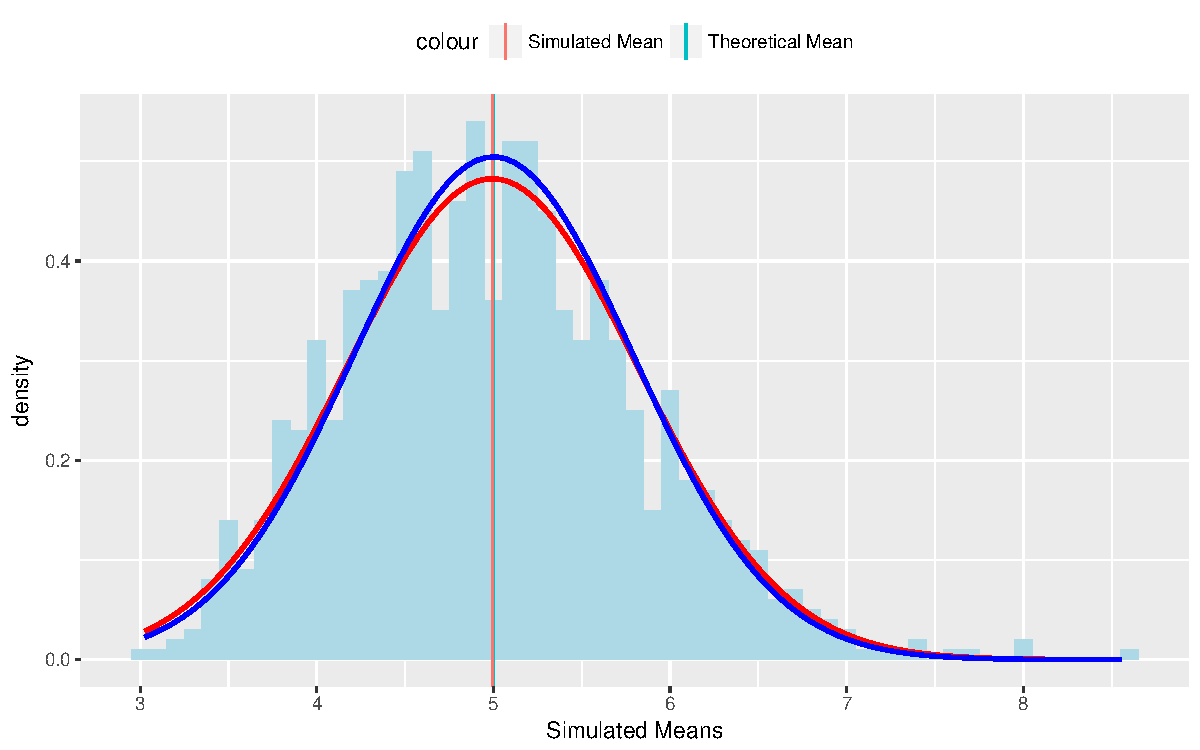
\includegraphics[width=\maxwidth]{figure/density-1} \caption[Distribution of the simulated means]{Distribution of the simulated means}\label{fig:density}
\end{figure}


\end{knitrout}


\begin{knitrout}
\definecolor{shadecolor}{rgb}{0.969, 0.969, 0.969}\color{fgcolor}\begin{kframe}
\begin{alltt}
\hlcom{# use qqplot and qqline to compare the distribution of averages of 40 exponentials}
\hlcom{# to a normal distribution}
\hlkwd{qqnorm}\hlstd{(simMeans)}
\hlkwd{qqline}\hlstd{(simMeans,} \hlkwc{col} \hlstd{=} \hlnum{2}\hlstd{)}
\end{alltt}
\end{kframe}\begin{figure}
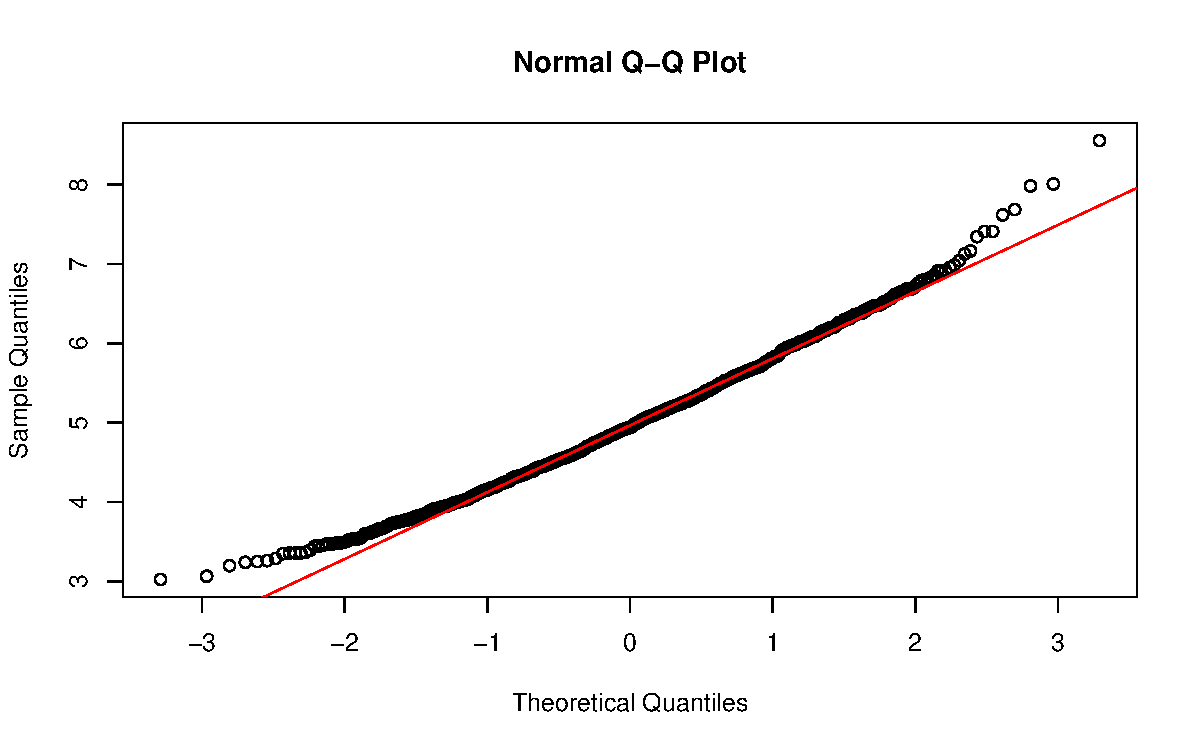
\includegraphics[width=\maxwidth]{figure/qqplot-1} \caption[The points lie mostly on the line so the distribution has the same shape as the thoretical distribution]{The points lie mostly on the line so the distribution has the same shape as the thoretical distribution}\label{fig:qqplot}
\end{figure}


\end{knitrout}

  
\end{document}
